\section*{سوال ۱}

مفهوم
\lr{AMI}
یا
\lr{Ambient Intelligence}
چیست و آینده آن به چه صورتی است؟

\section*{جواب سوال ۱}

\begin{figure}[H]
	\centering
	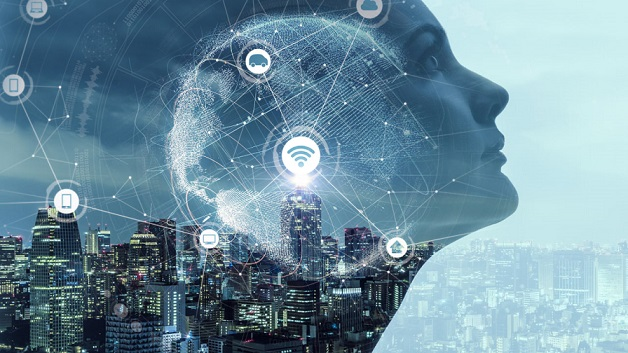
\includegraphics{pic1.jpg}
	\label{fig:label4}
\end{figure}

\lr{Ambient Intelligence (AMI)}
به فناوری و محیطی اشاره دارد که در آن ابزارهای الکترونیکی، سنسورها، دستگاه‌های اکتواتور (موتورهای کوچک برای حرکت یا کنترل محیط) و فناوری‌های پیشرفته دیگر، به طور پیوسته، در هم تنیده و متصل هستند تا یک محیط زنده و هوشمند ایجاد کنند. در این محیط، تکنولوژی به گونه‌ای با زندگی روزمره ادغام شده است که کاربران به صورت تقریباً نامحسوس از آن بهره‌مند می‌شوند. این امکان را به افراد می‌دهد تا بدون نیاز به فهم پیچیدگی‌های فنی، با دستگاه‌های اطراف خود به طور طبیعی تعامل داشته باشند.

\section*{پیشینه AMI}
مفهوم
\lr{AMI}
در دهه 1990 توسعه یافت، زمانی که موسسات تحقیقاتی مانند
\lr{Philips}
و
\lr{MIT Media Lab}
شروع به کاوش در فناوری‌هایی کردند که می‌توانستند به صورت پیوسته و بدون دخالت آشکار کاربر، در زندگی روزمره او تأثیر بگذارند. با پیشرفت‌های سریع در فناوری‌های ارتباطی و شبکه‌ای، ایده‌هایی مانند خانه‌های هوشمند و شهرهای هوشمند به تدریج به واقعیت نزدیک شدند.

\begin{figure}[H]
	\centering
	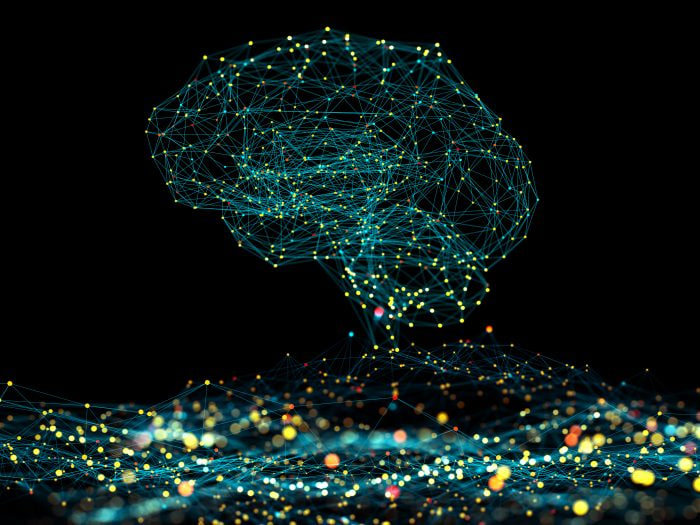
\includegraphics{pic2.jpg}
	\label{fig:label4}
\end{figure}

\section*{حال حاضر و آینده AMI}
در حال حاضر،
\lr{AMI}
در حال پیدا کردن جایگاهی است در بسیاری از جنبه‌های زندگی مدرن، از خانه‌های هوشمند گرفته تا محیط‌های کاری و حتی شهرهای هوشمند. با گسترش اینترنت اشیاء 
\lr{(IoT)}
و فناوری‌های مانند هوش مصنوعی و یادگیری ماشین، این سیستم‌ها به طور فزاینده‌ای می‌توانند اقدامات و نیازهای انسانی را پیش‌بینی کنند و به آنها پاسخ دهند.

آینده‌ی
\lr{AMI}
می‌تواند شامل پیشرفت‌های چشمگیری باشد، از جمله:
\begin{itemize}
	\item انطباق‌پذیری بیشتر: محیط‌ها به طور فعال با نیازها و ترجیحات افراد سازگار خواهند شد.
	\item پیشرفت‌های در حوزه حریم خصوصی و امنیت: با افزایش نگرانی‌های مربوط به داده‌های شخصی، فناوری‌های جدید باید به گونه‌ای طراحی شوند که حفظ حریم خصوصی را تضمین کنند.
	\item همگرایی بیشتر با پوشیدنی‌ها: دستگاه‌های پوشیدنی همچنان با محیط اطراف ادغام خواهند شد، اجازه دادن به کاربران برای انجام تعاملات پیچیده تر با محیط.
	\item استقلال و خودمختاری: سیستم‌های \lr{AMI} ممکن است قادر به انجام تصمیم‌گیری‌های پیچیده‌تر بدون نیاز به دخالت انسانی باشند.
	\item تعاملات انسان-ماشین طبیعی‌تر: با پیشرفت در زمینه شناسایی گفتار و پردازش زبان طبیعی، تعامل با سیستم‌های \lr{AMI} بیش از پیش طبیعی و انسانی خواهد شد.
\end{itemize}
این فناوری‌ها نه تنها زندگی روزمره را آسان‌تر می‌کنند، بلکه می‌توانند برای کمک به افراد معلول، سالمندان و دیگر گروه‌های آسیب‌پذیر در جامعه به کار روند.

\section*{کاربردهای عملی \lr{AMI}}
توضیح دهید که چگونه \lr{AMI} در زمینه‌های مختلفی مانند مراقبت‌های بهداشتی، حمل و نقل، صنعت خرده‌فروشی و مدیریت انرژی به کار می‌رود.

\section*{تأثیر \lr{AMI} بر تجربه کاربر}
بحث کنید که چگونه \lr{AMI} می‌تواند تجربه کاربری را شخصی‌سازی کرده و از طریق تجزیه و تحلیل رفتار، پیشنهادات و خدمات بهتری ارائه دهد.

\section*{مسائل اخلاقی و حریم خصوصی}
بررسی کنید که چگونه جمع‌آوری و پردازش داده‌های شخصی توسط سیستم‌های \lr{AMI} می‌تواند به مسائل اخلاقی و نگرانی‌هایی در مورد حریم خصوصی منجر شود و چه راهکارهایی می‌توان ارائه داد.

\section*{چالش‌های امنیتی}
توضیح دهید که چگونه امنیت سایبری برای حفاظت از سیستم‌های \lr{AMI} در برابر حملات و نقض داده‌ها ضروری است.

\section*{تکنولوژی‌های پیشران}
معرفی و توضیح فناوری‌های کلیدی که \lr{AMI} را امکان‌پذیر می‌سازند، مانند شبکه‌های حسگر بی‌سیم، هوش مصنوعی، محاسبات ابری، و اینترنت اشیاء.

\section*{پیشرفت‌های آتی}
پیش‌بینی کنید که چگونه پیشرفت‌های فناوری ممکن است ظهور \lr{AMI} را در آینده تغییر دهند و چه نوآوری‌هایی ممکن است به وجود آیند.

\section*{مطالعات موردی}
مثال‌های واقعی از سیستم‌های \lr{AMI} را که هم‌اکنون در استفاده هستند بیاورید و نحوه تأثیر آن‌ها بر زندگی روزمره را تشریح کنید.

\section*{طراحی و معماری سیستم‌های \lr{AMI}}
بررسی کنید که طراحان چگونه باید عوامل انسانی را در نظر بگیرند و سیستم‌هایی بسازند که هم هوشمند و هم کاربرپسند باشند.

\section*{تأثیر اجتماعی و فرهنگی}
نحوه تأثیرگذاری \lr{AMI} بر جوامع و فرهنگ‌ها را بررسی کنید و چالش‌های اجتماعی ناشی از این فناوری‌ها را مورد نقد قرار دهید.

\section*{توسعه پایدار و \lr{AMI}}
نقش \lr{AMI} را در ترویج توسعه پایدار و مدیریت منابع طبیعی به صورت مؤثرتر مورد بحث قرار دهید.
	